\documentclass{wyrmtongue-oct}
\usepackage[utf8]{inputenc}
\usepackage{xifthen}
\usepackage[super]{nth}
\usepackage{xcolor}
\usepackage{hyperref}

\hypersetup{
    colorlinks=true,
    linkcolor=black,
    citecolor=black,
    urlcolor=blue,
    citecolor = blue,
    anchorcolor = blue
}

\begin{document}
% \thispagestyle{empty}
% \begin{center}
%     % 
\includegraphics[width=\textwidth]{img/profile/placeholder.png}
%     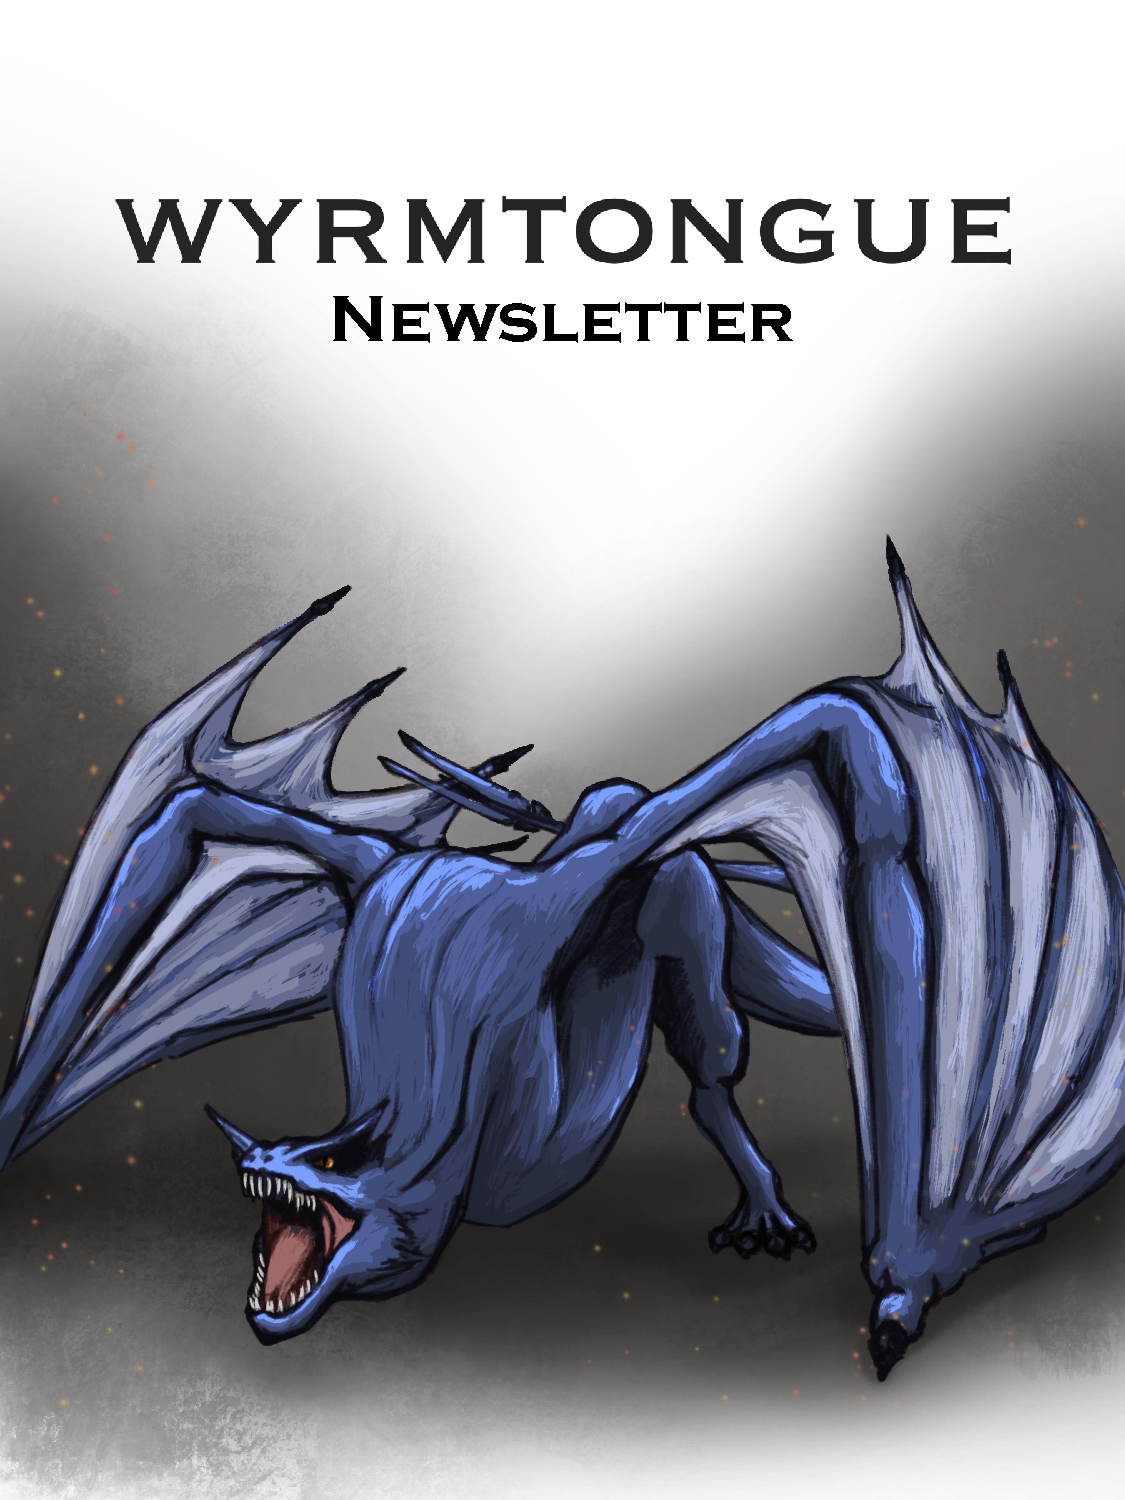
\includegraphics[width=\linewidth]{img/newsletter-cover-no-logo-2024.pdf}
% \end{center}
% \par\vspace{\fill}
% \begin{center}
%   
\includegraphics[width=0.4\textwidth]{img/logo/logo-alt.png}
% \end{center}

\begin{titlepage}
    \AddToShipoutPictureBG*{%
              \AtPageLowerLeft{%
                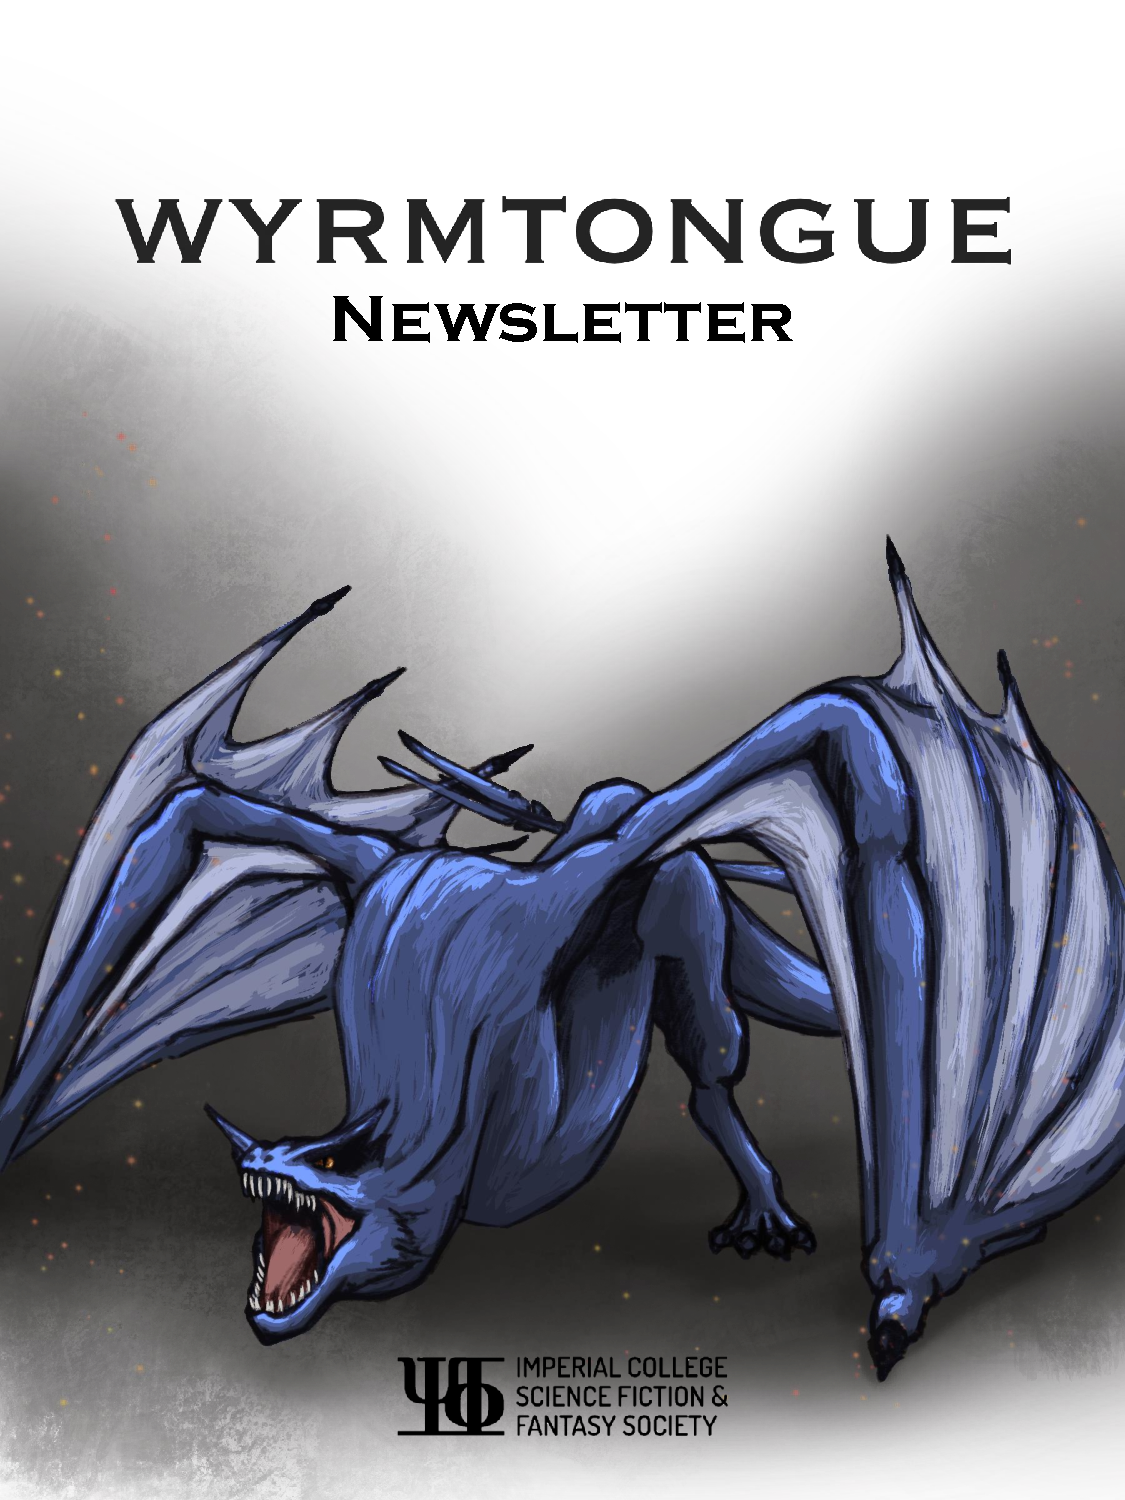
\includegraphics[width=\paperwidth,height=\paperheight]{img/newsletter-cover-2024.pdf}%
              }%
            }
\end{titlepage}

\textbf{      } % this is so hacky

\clearpage
\setcounter{page}{1}

\tableofcontents
\clearpage

% \pagehead{README}
To the unfortunate souls who chose to work on this mess of a template, here's what you need to do:

\begin{enumerate}
    \item Navigate to the \verb|txt| folder. You should find a .tex file named after your role. Type your stuff on there.
    \item Once that's done, pick an appropriate profile picture and head to the \verb|profile| folder under \verb|img|. Rename your picture with one of the png file names and replace it.
    \item Go to \verb|main.tex| and replace ``placeholder" with the appropriate tag in your section ie ``chair" or ``librarian"
\end{enumerate}

Note: If you face any issues, please harass the dumbass who got elected to be editor this year. Happy \LaTeX ing :)\
\clearpage

\article{editor}{From the Editor}
{Clifford Chan}{Editor}
\footnotetext[2]{This is not a joke. We will slap you with raw salmon.}
\clearpage

\article{chair}{Captain's Log}
{Hazel Wright}{Chair Entity}
\footnotetext[2]{Usually.}
\clearpage

\article{librarian}{Welcome to the Library!}
{Hetty Symes}{Head Librarian}
\clearpage

To give you some ideas about what to take out of the library, here are some recommendations from the committee members of books to borrow:

\newcommand{\bookrec}[4]{\noindent
  {#1}\newline
  \indent \textemdash{} \altfont{\textbf{#2}} by {#3}\newline
  \indent \textit{#4}
}

{ \bookrec
  {Henry Wild}
  {Kings of the Wyld}
  {Nicholas Eames}
  {Fantasy mercenary bands treated like musical bands.}
}

{ \bookrec
  {Connor Winzar}
  {
    Injustice: Gods Among Us\footnote{
      This is a comic. We have those.
    }
  }
  {Tom Taylor and Brian Buccellato}
  {A story of the corruption of Superman's morals and his descent into tyranny.}
}

{ \bookrec
  {Michael Figini}
  {The Simpsons and their Mathematical Secrets\footnote{
      This is a non-fiction book. We have those too.
    }
  }
  {Simon Singh}
  {Makes you want to re-watch the show just to find the mathematical secrets.}
}

{ \bookrec
  {Matthew Legg}
  {The Hitchhiker's Guide to the Galaxy}
  {Douglas Adams}
  {Earth has been demolished. Don't Panic, and please don't forget to bring your towel.}
}

{ \bookrec
  {Matthew Last}
  {Mort}
  {Terry Pratchett}
  {Death gets an apprentice. A strong introduction to the Discworld series.}
}

{ \bookrec
  {Edward Pickup}
  {The Red Knight}
  {Miles Cameron}
  {Fantasy Britain, but the Scottish are demons.}
}

{ \bookrec
  {Harry Black}
  {Speaker for the Dead}
  {Orson Scott Card}
  {Aliens, philosophy, and psychology?}
}

{ \bookrec
  {Jean Lo}
  {Schild's Ladder}
  {Greg Egan}
  {Differential geometry as a metaphor for character development.}
}

{ \bookrec
  {Sequoia Trevorrow}
  {
    The Songs of Distant Earth\footnote{
      Sequoia also recommends the album of the same name, by Mike Oldfield.
    }
  }
  {Arthur C. Clarke}
  {Earth is gone. God is dead. Life is still an emotion-filled rollercoaster.}
}

{ \bookrec
  {Timothy Davison}
  {Foundation}
  {Isaac Asimov}
  {The Empire is crumbling. Fight the chaos.}
}

\clearpage

\article{events}{Events Timetable}
{Sam Shenker}{Chair of Vice\\(Events Officer)}
\clearpage

% Would the publicity officer(Michelle) need a page?

% \begin{calendar}{October}
  \calendarhead
  \calendarweek{
    \calendarday[29]{}
    &\calendarday{\calendarevent{ICSF Library}{Literary Lucky Dip\footnotemark[2]}{}}
    &\calendarday[1]{}
    &\calendarday{\calendarevent{12:00-20:00 ICSF Library}{Wanna-Go Wednesday}{}}
    &\calendarday{\calendarevent{18:00-24:30 Blackett 1004}{Meet and Greet}{}}
    &\calendarday{\calendarevent{}{Themed Friday}{Blockbuster Night}}
    &\calendarday{}
  }
  \calendarweek{
    \calendarday{}
    &\calendarday{}
    &\calendarday{}
    &\calendarday{}
    &\calendarday{}
    &\calendarday{\calendarevent{}{Themed Friday}{Infinity War / Endgame}}
    &\calendarday{}
  }
  \calendarweek{
    \calendarday{}
    &\calendarday{}
    &\calendarday{}
    &\calendarday{\calendarevent{}{EGM\footnotemark[3]}{}}
    &\calendarday{}
    &\calendarday{\calendarevent{}{Cinema Trip}{Zombieland: Double Tap}}
    &\calendarday{}
  }
  \calendarweek{
    \calendarday{}
    &\calendarday{}
    &\calendarday{}
    &\calendarday{}
    &\calendarday{\calendarevent{}{Bar Night}{}}
    &\calendarday{}
    &\calendarday{\calendarevent{}{Book Crawl}{}}
  }
\end{calendar}

\begin{calendar}{November}
  \calendarhead
  \calendarweek{
    \calendarday{}
    &\calendarday{}
    &\calendarday{}
    &\calendarday{}
    &\calendarday{}
    &\calendarday[1]{\calendarevent{18:00-23:00 Dyson Library}{Halloween Party}{}}
    &\calendarday{}
  }
  \calendarweek{
    \calendarday{}
    &\calendarday{}
    &\calendarday{}
    &\calendarday{}
    &\calendarday{}
    &\calendarday{}
    &\calendarday{}
  }
  \calendarweek{
    \calendarday{}
    &\calendarday{}
    &\calendarday{}
    &\calendarday{}
    &\calendarday{}
    &\calendarday{}
    &\calendarday{}
  }
  \calendarweek{
    \calendarday{}
    &\calendarday{}
    &\calendarday{}
    &\calendarday{}
    &\calendarday{}
    &\calendarday{\calendarevent{}{Themed Friday}{Doctor Who}}
    &\calendarday{}
  }
\end{calendar}

\vspace{\fill}

\begin{center}
  \begin{minipage}{0.65\textwidth}
    \itshape
  Regular lunchtime showings (every weekday!) continue throughout
  term-time. Unofficial events not listed.

  More to be announced as we go! Subscribe to our mailing lists to
  receive the latest updates.
\end{minipage}
\end{center}

\vspace{\fill}

% \footnotetext[2]{Continues into the week --- drop by the library whenever
%   and pick up a mystery book.}
% \footnotetext[3]{Themed Fridays usually start at 18:00 in the Library.}
% \footnotetext[4]{Extraordinary General Meeting. Run for a committee position!}
\clearpage

\article{picocon}{Picocon}
{Juairiyah Raqib}{Picocon Sofa\footnotemark[2]}
\footnotetext[2]{Like a chair, but comfier\texttrademark{}}
\clearpage

\pagehead{Picocon Sneak Peek!!}

\begin{center}
    
\includegraphics[height=\textwidth]{img/profile/placeholder.png}
\end{center}

We also publish a collection of short stories, artwork and poetry in conjunction with Picocon! This year's theme is \textit{???}. If you wish to contribute to the fanzine, submit your work to \texttt{icsfwyrmtongue@gmail.com}\footnotemark[2]. 

\footnotetext[2]{Submissions will be open from start of Spring term until the end of February.}
\clearpage

% \pagehead{Whispers from the Basement}

Imperial College Science Fiction and Fantasy Society brings their
weird and wonderful conversations directly to your auditory organs!
Tune in for an hour of terrible banter, mysterious music, and
life-changing revelations in dialogue.

\textit{Whispers from the Basement} airs every Wednesday afternoon
14:00--15:00 on IC Radio. Find updates about the show and listen to
previous broadcasts on the IC Radio website
at \texttt{icradio.com/shows/1016/}.

% \par\vspace{\fill}
\pagehead{Getting Involved}

\subhead{Mailing Lists}

ICSF maintains the following mailing lists, to which all members are welcome to
subscribe:

\begin{itemize}
\item \texttt{icsf-list}
is the society’s core mailing list, which communicates announcements
of ICSF events and important news about the society. This list does
not generate an overwhelming amount of traffic, and subscription is a
must if you would like to hear about film trips and other activities.

% \item \texttt{icsf-committee}
% is our ‘management’ list --- but it gets used a lot more
% widely than that. Here you’ll be able to contribute your opinion to
% the running of the society.
\end{itemize}

% QR code for mailing list
\begin{minipage}[h]{7.8em}

\includegraphics[height=\textwidth]{img/info/qr-mailing-list.png}
\end{minipage}
\begin{minipage}[h]{0.82\linewidth}
\raggedright
Join our mailing list by scanning the QR code. Alternatively, subscribe automatically by signing up for membership at: 
\href{https://www.imperialcollegeunion.org/activities/a-to-z/science-fiction-and-fantasy}{www.imperialcollegeunion.org/activities/a-to-z/science-fiction-and-fantasy}.
\end{minipage}

\subhead{Social Media}
For those who welcome our social network overlords, behold
continuations of the Library into the realms of cyberspace:

\socialmedia{facebook}{\href{https://www.facebook.com/groups/ICSF.imperial}{facebook.com/groups/ICSF.imperial}}{
Sci-fi talk, news and events, amusing links.
}

% \socialmedia{twitter}{@Picocon}{
% Announcements and excitement for our annual convention.
% }

\socialmedia{twitter}{\href{https://twitter.com/Imperial_SciFi}{@Imperial\_SciFi}}{
Sci-fi and fantasy, 280 characters at a time.
}

\socialmedia{instagram}{\href{https://www.instagram.com/imperial_scifi/?hl=en}{@imperial\_scifi}}{
Visions from the library, visions from the future (event announcements).
}

\par\vspace{\fill}
\clearpage

% \pagehead{\LARGE Book review -- Neuromancer by William Gibson}
Things to write here...
% \tombstone
% \clearpage

% \vfill
\begin{Puzzle}{13}{13}
|[1]C |O |[2]S |M |I    |[3]C |*  |[4]N |A     |V |[5]A |N |[6]I |.
|A    |* |Q    |* |*    |R    |*  |O    |*     |* |B    |* |S    |.
|[7]D |O |U    |B |L    |E    |*  |[8]V |A     |N |D    |A |L    |.
|M    |* |I    |* |*    |E    |*  |I    |*     |* |U    |* |A    |.
|U    |* |R    |* |[9]S |P    |I  |C    |[10]E |* |C    |* |N    |.
|[11]S|L |E    |E |P    |Y    |*  |[12]E|X     |I |T    |E |D    |.
|*    |* |*    |* |A    |*    |*  |*    |T     |* |*    |* |*    |.
|[13]S|P |[14]R|A |W    |[15]L|*  |[16]F|R     |O |[17]Z|E |[18]N|.
|U    |* |A    |* |[19]N|I    |N  |J    |A     |* |O    |* |E    |.
|N    |* |C    |* |*    |S    |*  |O    |*     |* |M    |* |W    |.
|[20]S|P |O    |I |L    |T    |*  |[21]R|U     |B |B    |L |E    |.
|E    |* |O    |* |*    |E    |*  |D    |*     |* |I    |* |S    |.
|[22]T|I |N    |T |I    |N    |*  |[23]S|T     |R |E    |E |T    |.
\end{Puzzle}

\newcommand{\blnk}{\underline{\hspace{2em}}}

\newcommand{\cwclue}[4]{
% #1 - number
% #2 - answer
% #3 - question
% #4 - length
\item[\texttt{#1}] {{#3} ({#4})}
}
\hfill
\begin{minipage}[t]{0.45\textwidth}
\begin{center}{\large \altfont{Across}}\end{center}
\begin{small}
\begin{itemize}[leftmargin=*,topsep=0pt,itemsep=0pt]
\cwclue{ 1}{COSMIC}{The Fantastic Four gained their powers through \blnk rays}{6}
\cwclue{ 4}{NAVANI}{Renowned Brightlady and Artifabrian}{6}
\cwclue{ 7}{DOUBLE}{Prepare for trouble, and make it \blnk}{6}
\cwclue{ 8}{VANDAL}{\blnk Savage, immortal supervillain}{6}
\cwclue{ 9}{SPICE}{The only thing of worth on Arrakis}{5}
\cwclue{11}{SLEEPY}{What the Silmarillion makes most people}{6}
\cwclue{12}{EXITED}{The  Pevensies \blnk our world through a wardrobe}{6}
\cwclue{13}{SPRAWL}{Colloquial name for the setting of \emph{Neuromancer}, \emph{Count Zero} and \emph{Mona Lisa Overdrive}}{6}
\cwclue{16}{FROZEN}{Disney's version of \emph{The Snow Queen}}{6}
\cwclue{19}{NINJA}{Japanese covert agent}{5}
\cwclue{20}{SPOILT}{Joffrey Baratheon in a nutshell}{6}
\cwclue{21}{RUBBLE}{The Vogons turned the Earth to this}{6}
\cwclue{22}{TINTIN}{Belgium's greatest reporter and adventurer}{6}
\cwclue{23}{STREET}{221B Baker \blnk }{6}
\end{itemize}
\end{small}
\end{minipage}
\hfill
\begin{minipage}[t]{0.45\textwidth}
\begin{center}{\large \altfont{Down}}\end{center}
\begin{small}
\begin{itemize}[leftmargin=*,topsep=0pt,itemsep=0pt]
\cwclue{ 1}{CADMUS}{Founder of Thebes and creator of Superboy}{6}
\cwclue{ 2}{SQUIRE}{Podrick Payne was Tyrion Lannister's \blnk in \emph{A Song of Ice and Fire}}{6}
\cwclue{ 3}{CREEPY}{The Uncanny Valley}{6}
\cwclue{ 4}{NOVICE}{A wizard's apprentice}{6}
\cwclue{ 5}{ABDUCT}{What aliens do to cows every other Thursday}{6}
\cwclue{ 6}{ISLAND}{Roke, Azkaban, Númenor}{6}
\cwclue{ 9}{SPAWN}{Star-\blnk of Cthulhu}{5}
\cwclue{10}{EXTRA}{E.T. The \blnk-Terrestrial}{5}
\cwclue{13}{SUNSET}{Tatooine has two of these each day}{6}
\cwclue{14}{RACOON}{Bradley Cooper's Space Rocket}{6}
\cwclue{15}{LISTEN}{Hey! \blnk! : Navi}{6}
\cwclue{16}{FJORDS}{Pining for the \blnk}{6}
\cwclue{17}{ZOMBIE}{Classic Apocalypse}{6}
\cwclue{18}{NEWEST}{Jodie Whittaker is the \blnk Doctor}{6}
\end{itemize}
\end{small}
\end{minipage}
\hfill
\vfill

% \clearpage

\thispagestyle{empty}
% there is no esoteric meaning in the strangely specific numbers. It
% was 3AM on the day before printing and I was eyeballing all the
% dimensions.
\vspace*{\fill}

\hspace{\fill}%
\begin{minipage}{\textwidth}
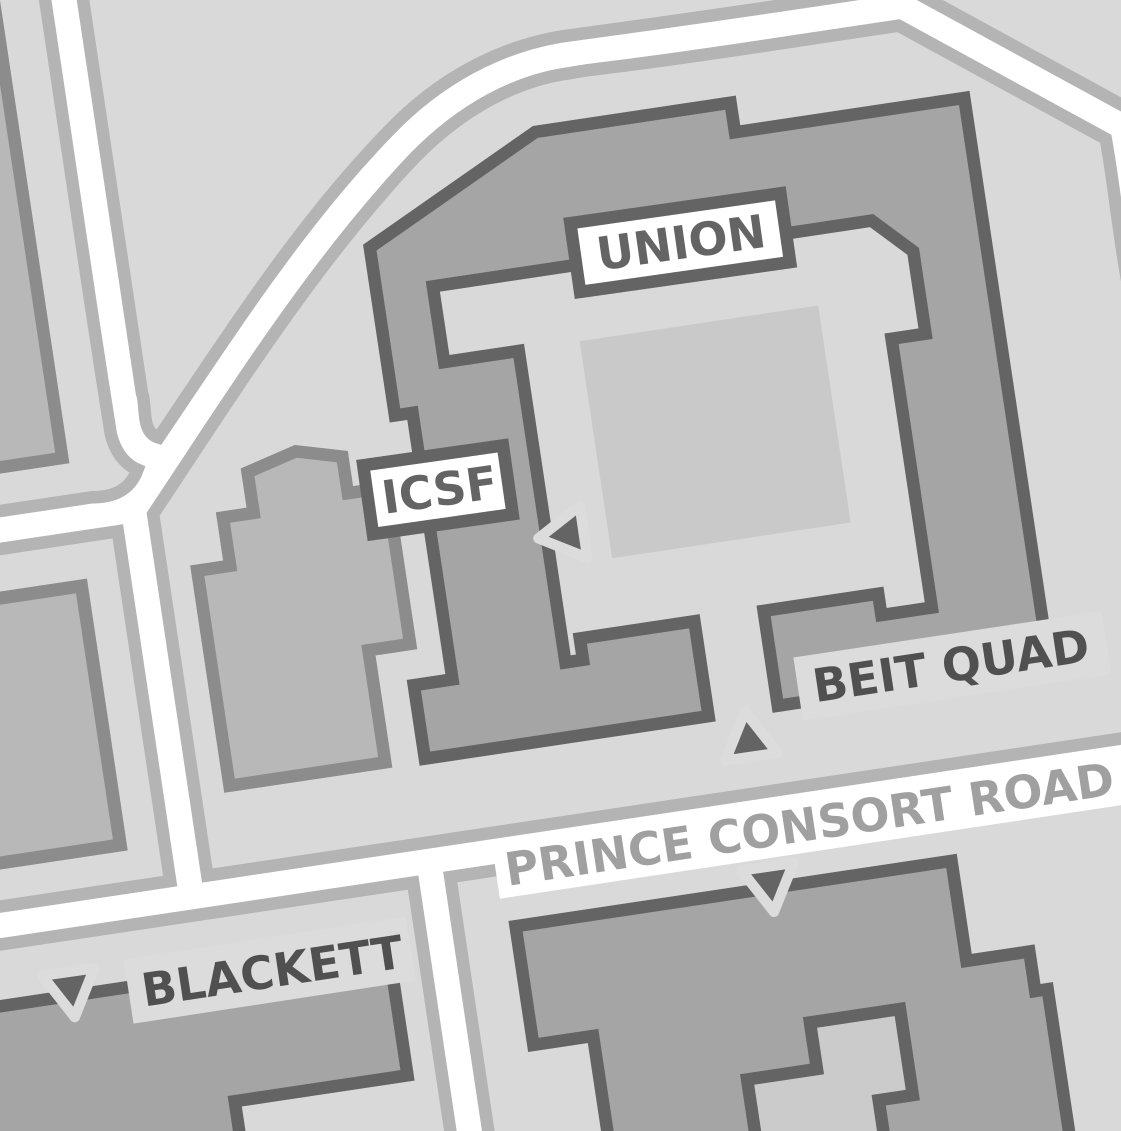
\includegraphics[width=\textwidth]{img/info/map.png}

\vspace{2em}

% QR code for membership
\begin{minipage}[h]{7.8em}

\includegraphics[height=\textwidth]{img/info/qr-small.png}
\end{minipage}%
\hspace{1.5em}%
% logotext
\begin{minipage}[h]{12em}
\raggedright

\includegraphics[width=\textwidth]{img/logo/logo-text.png}
Published November~2023
\texttt{icsf.org.uk}
\end{minipage}
\hspace*{\fill}%
\end{minipage}

\clearpage

\end{document}
